\section{Comparison across Hosted Deployments}
\label{app:hosted-comparison}

Figure~\ref{fig:hosted-verified-breadth} compares accuracy and success-conditional
solution-mode diversity across hosted deployments. Its accuracy row uses a
common formatting normalizer and the revised Opus 5 \texttt{Python} instructions at
each level; hollow marks show that deployment's original \texttt{Python} condition.
Other accuracy cells use the original instructions. The diversity row uses
strict grades and original instructions for every deployment, with the
prompt-level estimand and eligibility criteria of App.~\ref{app:hosted-mode-diversity}.
Accuracy includes every response, including refusals and verification failures.
Provider settings differ, so the figure describes the stated configurations
rather than ranking models under matched prompts and compute.

The tables and \texttt{Graph} figure use the original instructions for every deployment.
The \texttt{Python} comparison reports both instruction conditions under strict and
formatting-normalized grading. Level 3 extends the evaluation beyond the
training levels, and difficulty need not increase with level for every hosted deployment.

\paragraph{Evaluation population.}
The deployments are GPT-5.6 Sol, Claude Opus 5, GPT-5.4, Grok 4.3, Kimi K3, Claude Opus 4.8, DeepSeek V4 Pro. The original-instruction cohort contains
107,520 responses: 15,360 per deployment, with the same 128 held-out
prompts in each of five domains and three levels, and eight stateless responses
per prompt. Requests use no model-side tools or conversation history, and
the evaluation includes no task training or replay intervention.

\paragraph{Provider configurations.}
All deployments request medium reasoning effort and an 8,192-token native
output limit. Claude Opus 5 and Claude Opus 4.8 use Anthropic Messages with
adaptive thinking; the other deployments use hosted API routes.

The requested reasoning setting and output limit do not match compute across
providers: effort labels and token accounting have provider-specific meanings.
Temperature and nucleus sampling use provider defaults, whose exact values
are unknown when the provider does not return them.

Strict grading checks the original executable answer; formatting-normalized
grading applies the same typography corrections across deployments before
the executable checks. The tables below report original-instruction results
under both grading rules. Prompt preferences and the Level-1 \texttt{PantryPlan}
interface difference limit comparisons across levels. \texttt{Countdown} has no uniform
reference, because its total support is not certified. This inference-only comparison does not identify a training
cause, a model-size effect, or a difficulty effect. Collision intervals are
pointwise estimates for individual cells, not intervals for paired deployment differences.

The 15,360 scored DeepSeek V4 Pro responses include verification failures
and truncations. Usage totals omit requests without reported usage and
therefore give only a lower bound on the true total cost of all attempted API requests.

\begin{figure}[!htbp]
  \centering
  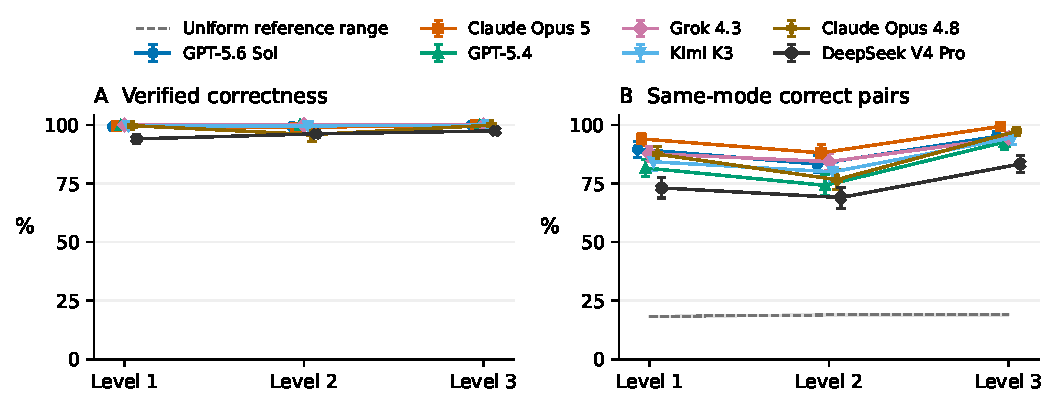
\includegraphics[width=\linewidth]{figures/frontier_comparison_20260911_graph.pdf}
  \caption{\textbf{Hosted \texttt{Graph} answers are usually correct but concentrated relative to uniform sampling.}
  Panel A shows strict per-response accuracy; panel B shows the fraction of
  correct pairs sharing a solution mode, pooling pairs across prompts. Colors
  and markers identify seven deployments, each with the same 128 prompts per
  level and eight stateless responses per prompt. Error bars are pointwise
  95\% intervals from resampling whole prompts. The gray band spans the
  deployments' uniform-correct-mode references, weighted by
  correct-pair counts; the dashed line is their mean. Level labels imply
  neither equal nor monotone difficulty across deployments.}
  \label{fig:hosted-graph-comparison}
\end{figure}

\subsection{A separate Python prompt sensitivity test}
\label{app:hosted-python-prompt}
After the original Opus 5 Python refusals, synthetic tasks were used to select
a direct arithmetic-expression formulation with no system message. We then
collected eight independent draws for every original Python test task: all
384 prompts across three levels, with unchanged adaptive thinking, medium
effort, 8,192 output tokens, allowed operators, public inputs and frozen graders.
The revised user instruction asks for a one-line boxed Python lambda returning
any proper divisor for each listed input. It does not prescribe a preferred divisor.
Both task wording and system-message presence change; collection time also differs.
This exploratory follow-up therefore supports a practical prompt repair without
isolating its cause. Original refusals and all three residual refusals are retained.
The original-protocol appendix tables retain all original Python responses;
the main display uses this complete revised condition with an explicit caption note.

\begin{table}[!htbp]
  \centering
  \caption{\textbf{Opus 5 Python: original versus plain task wording.}
  Each row has 1,024 responses. R counts native refusals; A is per-response accuracy (\%),
  D is \texttt{distinct@8}, and C is correct-pair collision (\%).
  Strict and normalized results use the same frozen grader and typography rule.
  Original Level-2/3 collision is undefined because no prompt has two correct draws.}
  \small
  \setlength{\tabcolsep}{4pt}
  \begin{tabular}{@{}llrrrrrrr@{}}
    \toprule
    & & & \multicolumn{3}{c}{Strict} & \multicolumn{3}{c}{Normalized} \\
    Condition & L & R & A & D & C & A & D & C \\
    \midrule
    Original & 1 & 409 & 38.1 & 0.91 & 93.0 & 60.0 & 1.12 & 90.4 \\
     & 2 & 1021 & 0.3 & 0.02 & -- & 0.3 & 0.02 & -- \\
     & 3 & 1024 & 0.0 & 0.00 & -- & 0.0 & 0.00 & -- \\
    \midrule
    Plain user, no system & 1 & 0 & 74.9 & 1.42 & 80.2 & 100.0 & 1.49 & 79.9 \\
     & 2 & 0 & 71.8 & 1.31 & 84.7 & 100.0 & 1.38 & 85.7 \\
     & 3 & 3 & 76.2 & 1.38 & 82.7 & 99.7 & 1.41 & 84.1 \\
    \bottomrule
  \end{tabular}
\end{table}

The new condition has no API failures or token-limit truncations. Strict grading
accepts 2,282 responses; the frozen rule rescues 787 more
by converting escaped percent signs (\verb|\%|) to Python modulo (\verb|%|).
Thus every non-refused answer passes after this formatting-only correction.
Normalized collision is 79.9/85.7/84.1\%, versus conditional uniform references
of 1.43/1.15/1.15\%. The residual three refusals occur on two prompts whose
other identical requests are accepted. No retry-until-accepted selection is used.

The paired analysis resamples whole eight-draw prompt groups across conditions
(20,000 replicates). Normalized accuracy gains at Levels 1/2/3 are
40.0 [34.7, 45.5], 99.7 [99.3, 100.0], and 99.7 [99.2, 100.0] percentage points
(pointwise 95\% intervals). Output draws themselves are independent, and the
different correct-pair populations preclude interpreting a raw collision
difference as a matched-population prompt effect.

The saved sensitivity record binds the original and revised native receipts,
request payloads, strict regrade audit and frozen normalization outputs.

\paragraph{Separate first-valid retry diagnostic.}
After completing the fixed 3,072-response revised-wording cohort, a separate
condition retries only its three remaining refused slots, retaining the
first verified-valid response. All three succeed on their first additional
request, and all reproduce a mode already seen for that prompt. This uses
3,075 requests to select 3,072 valid responses; its 100\% accepted-set
accuracy follows from selection and is not unconditional model accuracy.
The selected set's \texttt{distinct@8} is unchanged at 1.492, 1.375, 1.414 at
Levels 1--3. Level-3 correct-pair collision changes from 84.0909\% to 84.1518\%;
the other levels are unchanged. All initial and retry responses remain
preserved. The main figure continues to use the complete fixed eight-draw
condition, including its three refusals; these selected-validity results
are only a separate diagnostic with variable request effort.


\subsection{Requested-temperature sensitivity}
\label{app:hosted-temperature}
Grok 4.3 and Kimi K3 each receive requested temperatures $T=1.0$ and
$T=1.5$ on the same 120 tasks: eight prompts in each of five domains and
three levels. Eight responses from separate requests per prompt give 960
responses per deployment--temperature condition and 3,840 in total.
Within each deployment, the two conditions share all non-temperature
request settings and run concurrently. Accuracy and mode counts include
all responses, including verification failures and truncated outputs.

The providers accept both requested temperature settings, but their responses
do not report effective sampling temperatures. DeepSeek is outside this
comparison because its thinking-mode interface ignores the temperature setting.
The results concern these requested settings on this 120-task subset and
do not establish a general temperature response for all hosted deployments.

Each level summary averages five domains equally; All averages the 15
domain--level cells equally. Collision pools correct pairs within each cell,
so tasks with more correct responses receive more weight. Eligible tasks
and pair weights can differ between temperatures; the contrast does not
hold accuracy or the correct-pair population fixed. An undefined cell makes
the corresponding average undefined. Pointwise 95\% intervals use 20,000
paired whole-prompt bootstrap resamples, stratified by domain and level.
Each resampled prompt includes all eight responses. Prompts are paired
across conditions; output draws are not. Intervals have no multiplicity adjustment.

\paragraph{Observed sensitivity.}
For Grok, the observed diversity change is +0.050 [$-$0.058, +0.158] modes, and the collision change is $-$0.78 [$-$3.86, +2.12] percentage points. Both intervals include zero, so neither shows a clear diversity gain.
The per-response accuracy change is $-$2.29 [$-$3.85, $-$0.94] percentage points. These results do not establish invariance to temperature in general.

At $T=1.5$, 696 of Kimi's 960 outputs reach the token limit,
compared with 0 at $T=1.0$. Strict accuracy falls from 96.56\% to 21.25\%, while raw diversity falls from 1.933 to 0.983 modes.
The large increase in truncation accompanies losses in accuracy and distinct modes.
These results do not isolate correct-output concentration at matched accuracy.
The five-domain collision mean is undefined at
$T=1.5$ because some cells have no eligible correct pairs. Neither model
has provider-declared refusals in this experiment.

$\dagger$ marks a defined contrast whose interval is omitted because some
bootstrap resamples have undefined cells. Five-domain averages require all
five cell estimates; conditioning on only the estimable resamples would
change the uncertainty calculation.

\begin{table}[!htbp]
  \centering
  \setlength{\parfillskip}{0pt plus .20\linewidth}
  \caption{\textbf{Higher requested temperature yields no clear Grok diversity gain and much lower Kimi accuracy.} Strict executable grades compare $T=1.5$ with $T=1.0$.
  Each condition contains eight responses on each of 120 tasks.
  Level summaries average five domains equally; All averages 15 domain--level cells.
  A is per-response accuracy (\%); D is mean \texttt{distinct@8};
  C is correct-pair collision (\%), pooling pairs within each cell.
  Differences subtract $T=1.0$ from $T=1.5$: mode counts for D and percentage points for A/C.
  Brackets give pointwise 95\% intervals from paired whole-prompt bootstrap resampling.
  $\dagger$ marks an omitted interval when some resamples have undefined cells;
  -- denotes an undefined estimate or omitted interval.}
  \small
  \setlength{\tabcolsep}{5pt}
  \begin{tabular}{@{}llrrrr@{}}
    \toprule
    Deployment & Level & Metric & $T=1.0$ & $T=1.5$ & Difference [95\% interval] \\
    \midrule
    Grok 4.3 & 1 & A & 98.12 & 95.62 & $-$2.50 [$-$4.06, $-$0.94] \\
     &  & D & 1.900 & 2.000 & +0.100 [$-$0.100, +0.300] \\
     &  & C & 72.89 & 73.16 & +0.27 [$-$6.31, +6.37] \\
     & 2 & A & 99.06 & 99.38 & +0.31 [$-$0.94, +1.56] \\
     &  & D & 1.425 & 1.425 & +0.000 [$-$0.175, +0.200] \\
     &  & C & 86.61 & 85.20 & $-$1.41 [$-$6.26, +3.30] \\
     & 3 & A & 98.75 & 94.06 & $-$4.69 [$-$9.06, $-$0.94] \\
     &  & D & 1.500 & 1.550 & +0.050 [$-$0.125, +0.225] \\
     &  & C & 84.04 & 82.85 & $-$1.20 [$-$5.48, +2.79] \\
     & All & A & 98.65 & 96.35 & $-$2.29 [$-$3.85, $-$0.94] \\
     &  & D & 1.608 & 1.658 & +0.050 [$-$0.058, +0.158] \\
     &  & C & 81.18 & 80.40 & $-$0.78 [$-$3.86, +2.12] \\
    \midrule
    Kimi K3 & 1 & A & 92.50 & 22.50 & $-$70.00 [$-$75.62, $-$63.75] \\
     &  & D & 2.200 & 1.075 & $-$1.125 [$-$1.475, $-$0.775] \\
     &  & C & 66.23 & 53.12 & $-$13.11 [--]$^\dagger$ \\
     & 2 & A & 98.12 & 20.31 & $-$77.81 [$-$82.50, $-$72.81] \\
     &  & D & 1.850 & 0.900 & $-$0.950 [$-$1.300, $-$0.625] \\
     &  & C & 72.18 & 66.55 & $-$5.63 [--]$^\dagger$ \\
     & 3 & A & 99.06 & 20.94 & $-$78.12 [$-$83.75, $-$72.81] \\
     &  & D & 1.750 & 0.975 & $-$0.775 [$-$1.025, $-$0.525] \\
     &  & C & 78.33 & -- & -- \\
     & All & A & 96.56 & 21.25 & $-$75.31 [$-$78.44, $-$72.19] \\
     &  & D & 1.933 & 0.983 & $-$0.950 [$-$1.133, $-$0.767] \\
     &  & C & 72.25 & -- & -- \\
    \bottomrule
  \end{tabular}
\end{table}

\begin{table}[!htbp]
  \centering
  \setlength{\parfillskip}{0pt plus .20\linewidth}
  \caption{\textbf{Formatting normalization leaves the temperature sensitivity largely unchanged.} Only rows differing from strict grading appear; all other rows are identical.
  Each condition contains eight responses on each of 120 tasks.
  Level summaries average five domains equally; All averages 15 domain--level cells.
  A is per-response accuracy (\%); D is mean \texttt{distinct@8};
  C is correct-pair collision (\%), pooling pairs within each cell.
  Differences subtract $T=1.0$ from $T=1.5$: mode counts for D and percentage points for A/C.
  Brackets give pointwise 95\% intervals from paired whole-prompt bootstrap resampling.
  $\dagger$ marks an omitted interval when some resamples have undefined cells;
  -- denotes an undefined estimate or omitted interval.}
  \small
  \setlength{\tabcolsep}{5pt}
  \begin{tabular}{@{}llrrrr@{}}
    \toprule
    Deployment & Level & Metric & $T=1.0$ & $T=1.5$ & Difference [95\% interval] \\
    \midrule
    Kimi K3 & 1 & A & 92.50 & 22.81 & $-$69.69 [$-$75.31, $-$63.44] \\
     & 1 & C & 66.23 & 53.61 & $-$12.62 [--]$^\dagger$ \\
     & 3 & A & 99.38 & 20.94 & $-$78.44 [$-$84.06, $-$73.12] \\
     & 3 & C & 78.18 & -- & -- \\
     & All & A & 96.67 & 21.35 & $-$75.31 [$-$78.44, $-$72.19] \\
     & All & C & 72.20 & -- & -- \\
    \bottomrule
  \end{tabular}
\end{table}

Across the hosted comparisons, \texttt{Countdown} has no uniform reference because its
total support is not certified, so uniform-reference comparisons use the other
four domains. Cross-level differences
also reflect different task populations and do not establish a common ordering
of model difficulty. These inference-only results do not identify a training
or parameter-scale cause of concentration.


\subsection{GPT-5.6 Sol: temperature, pass@8 and verified modes}
\label{app:gpt56-temperature}
Figure~\ref{fig:gpt56-temperature-curve} plots empirical \texttt{pass@8}
against \texttt{distinct@8} for $T\in\{0.0,0.5,1.0,1.5,2.0\}$, with reasoning
\texttt{none}. Each condition uses the same 480 held-out prompts
(32 per domain--level cell), with eight stateless responses per prompt:
3,840 responses per temperature and 19,200 in total. A prompt contributes one
to \texttt{pass@8} if at least one of its eight answers is verified correct,
and contributes its number of distinct correct canonical keys to \texttt{distinct@8}.
Both metrics average over all prompts, including those with no correct answer.
The empirical \texttt{pass@8} uses the observed eight-response groups;
$1-(1-p)^8$ applied to pooled accuracy would ignore differences among prompts.
Raw \texttt{distinct@8} depends on both success and variation among correct
solution modes, so its changes need not track \texttt{pass@8}.

Prompts are selected independently of model outputs within each
domain--level cell. The evaluation comprises 120-prompt and 360-prompt
subsets collected at different times. Temperatures are interleaved for the
360-prompt subset; zero and nonzero temperatures are collected separately
for the 120-prompt subset. Service changes can therefore confound temperature
contrasts, and prompt composition can affect comparisons between subsets.

Requests use the same prompt wording, verifiers and sampling controls
except temperature, with an 8,192-token output cap. Returned metadata
identifies \texttt{gpt-5.6-sol-2026-07-09}, reasoning \texttt{none},
$\texttt{top\_p}=0.98$ and the requested temperature in every condition.
The exposed settings do not establish unchanged internal service behavior
or independent provider randomness. A zero-temperature request does not
establish deterministic outputs. The deployment rejects non-default
temperatures with medium reasoning and rejects temperature 2.5; this
sweep therefore does not test temperature robustness under medium reasoning.

Strict grading applies the executable validators directly. Normalized
grading uses the typography rules in App.~\ref{app:hosted-concentration}
before the same validators, preserving strict successes and their mode keys.

Each level averages five domains equally; All averages all 15 cells.
Pointwise 95\% intervals use 20,000 paired whole-prompt bootstrap
resamples stratified by domain and level, keeping all eight responses
together and matching prompts across temperatures. Individual model
responses are not paired across conditions.
There is no multiplicity adjustment. A zero-width empirical interval
reflects constant observed groups, not certain success on unseen prompts.

\begin{table}[!htbp]
\centering
\setlength{\parfillskip}{0pt plus .20\linewidth}
\caption{\textbf{Nonzero temperatures improve eight-draw coverage in this sweep.}
P is solved prompts (\%, \texttt{pass@8}); D is \texttt{distinct@8};
A is per-response accuracy (\%). G is the grading: S strict,
N formatting-normalized. Each temperature uses the same 480 prompts
(32 per domain--level cell), eight responses each, and reasoning \texttt{none}.
Level rows average five domains equally; All averages all 15 cells.
Brackets give pointwise 95\% whole-prompt bootstrap intervals.}
\label{tab:gpt56-temperature}
\small
\setlength{\tabcolsep}{4pt}
\begin{tabular}{@{}lllrrr@{}}
\toprule
$T$ & Level & G & P [95\% interval] & D [95\% interval] & A [95\% interval] \\
\midrule
0.0 & 1 & S & 55.0 [48.8, 61.3] & 0.569 [0.500, 0.637] & 53.9 [47.7, 60.1] \\
 & 2 &  & 45.0 [39.4, 50.6] & 0.456 [0.400, 0.512] & 39.5 [34.4, 44.7] \\
 & 3 &  & 49.4 [42.5, 56.2] & 0.519 [0.444, 0.594] & 44.5 [38.3, 50.9] \\
 & All &  & 49.8 [46.2, 53.3] & 0.515 [0.475, 0.554] & 46.0 [42.6, 49.4] \\
0.5 & 1 & S & 70.6 [64.4, 76.9] & 0.956 [0.850, 1.069] & 57.5 [51.9, 63.0] \\
 & 2 &  & 50.0 [44.4, 55.6] & 0.525 [0.463, 0.594] & 38.6 [33.9, 43.4] \\
 & 3 &  & 54.4 [48.1, 60.6] & 0.581 [0.506, 0.662] & 43.0 [37.1, 48.9] \\
 & All &  & 58.3 [54.8, 61.9] & 0.688 [0.640, 0.738] & 46.4 [43.3, 49.5] \\
1.0 & 1 & S & 75.6 [69.4, 81.2] & 1.181 [1.050, 1.312] & 57.3 [52.0, 62.7] \\
 & 2 &  & 51.9 [45.6, 58.1] & 0.581 [0.506, 0.662] & 37.6 [33.2, 42.0] \\
 & 3 &  & 60.6 [54.4, 66.9] & 0.713 [0.625, 0.806] & 42.7 [37.3, 48.1] \\
 & All &  & 62.7 [59.2, 66.2] & 0.825 [0.767, 0.885] & 45.9 [42.9, 48.8] \\
1.5 & 1 & S & 80.6 [75.0, 86.2] & 1.413 [1.269, 1.556] & 56.6 [51.7, 61.4] \\
 & 2 &  & 58.1 [51.9, 64.4] & 0.650 [0.569, 0.738] & 38.4 [34.3, 42.7] \\
 & 3 &  & 65.6 [59.4, 71.2] & 0.838 [0.731, 0.956] & 43.0 [38.0, 48.2] \\
 & All &  & 68.1 [64.8, 71.5] & 0.967 [0.900, 1.035] & 46.0 [43.3, 48.8] \\
2.0 & 1 & S & 83.8 [78.1, 88.8] & 1.519 [1.375, 1.663] & 59.7 [54.8, 64.5] \\
 & 2 &  & 54.4 [48.1, 60.6] & 0.600 [0.525, 0.675] & 35.3 [31.4, 39.3] \\
 & 3 &  & 61.9 [56.2, 67.5] & 0.819 [0.719, 0.925] & 40.5 [35.8, 45.5] \\
 & All &  & 66.7 [63.3, 70.0] & 0.979 [0.915, 1.044] & 45.2 [42.6, 47.8] \\
\midrule
0.0 & 1 & N & 70.6 [65.0, 76.2] & 0.725 [0.662, 0.788] & 70.5 [64.5, 76.2] \\
 & 2 &  & 60.6 [55.0, 66.2] & 0.613 [0.556, 0.669] & 54.5 [49.0, 59.9] \\
 & 3 &  & 65.6 [59.4, 71.9] & 0.681 [0.606, 0.756] & 61.4 [55.2, 67.6] \\
 & All &  & 65.6 [62.3, 69.0] & 0.673 [0.635, 0.710] & 62.1 [58.8, 65.5] \\
0.5 & 1 & N & 76.9 [71.2, 82.5] & 1.038 [0.931, 1.150] & 71.7 [66.4, 77.0] \\
 & 2 &  & 68.1 [62.5, 73.8] & 0.706 [0.644, 0.769] & 53.7 [48.8, 58.6] \\
 & 3 &  & 71.9 [65.6, 77.5] & 0.775 [0.700, 0.850] & 58.1 [52.3, 63.9] \\
 & All &  & 72.3 [69.2, 75.4] & 0.840 [0.792, 0.890] & 61.2 [58.2, 64.3] \\
1.0 & 1 & N & 79.4 [73.8, 84.4] & 1.238 [1.106, 1.369] & 70.4 [65.2, 75.5] \\
 & 2 &  & 69.4 [63.7, 75.0] & 0.756 [0.681, 0.831] & 51.6 [47.1, 56.2] \\
 & 3 &  & 76.9 [71.2, 82.5] & 0.894 [0.806, 0.988] & 55.2 [49.8, 60.7] \\
 & All &  & 75.2 [72.1, 78.3] & 0.963 [0.904, 1.021] & 59.1 [56.2, 62.0] \\
1.5 & 1 & N & 82.5 [77.5, 87.5] & 1.494 [1.344, 1.644] & 68.5 [63.7, 73.3] \\
 & 2 &  & 75.0 [69.4, 80.6] & 0.844 [0.762, 0.931] & 49.8 [45.5, 54.3] \\
 & 3 &  & 81.9 [76.2, 87.5] & 1.038 [0.931, 1.156] & 54.7 [49.6, 59.8] \\
 & All &  & 79.8 [76.7, 82.9] & 1.125 [1.056, 1.196] & 57.7 [54.9, 60.5] \\
2.0 & 1 & N & 85.0 [80.0, 90.0] & 1.606 [1.456, 1.762] & 69.6 [64.8, 74.3] \\
 & 2 &  & 72.5 [66.9, 78.1] & 0.800 [0.731, 0.869] & 45.7 [41.7, 49.8] \\
 & 3 &  & 80.6 [75.0, 86.2] & 1.031 [0.931, 1.137] & 52.5 [47.7, 57.5] \\
 & All &  & 79.4 [76.2, 82.5] & 1.146 [1.079, 1.212] & 55.9 [53.3, 58.6] \\
\bottomrule
\end{tabular}
\end{table}

\paragraph{Coverage and sampled solution modes.}
At $T=0.0$ and $T=2.0$, normalized \texttt{pass@8} is 65.62\% and 79.38\%, respectively,
while \texttt{distinct@8} is 0.673 and 1.146.
Across these five measured temperatures, the highest observed aggregate
\texttt{pass@8} occurs at $T=1.5$ and the highest \texttt{distinct@8}
occurs at $T=2.0$. These five temperatures do not establish
a population optimum or a continuous Pareto boundary, and level-specific curves differ.

Per-response accuracy changes from 62.11\% to 55.94\% between the endpoints.
That diagnostic is distinct from \texttt{pass@8}: success within eight
draws and the reliability of an individual draw need not change together as temperature varies.

The paired $T=2.0$ minus $T=0.0$ contrast is 13.8 [10.8, 16.7] \texttt{pass@8} percentage points and 0.473 [0.417, 0.529] distinct correct modes, with pointwise 95\% intervals.

\paragraph{Response outcomes.}
At every temperature, none of the 3,840 outputs is token-limited or a provider-declared refusal.
Unsuccessful answers remain in the eight-response groups.

\paragraph{Sensitivity across prompt subsets.}
We compare the same temperature contrast within each prompt subset.
The subsets differ in prompts and collection periods, so differences
between them do not isolate a causal effect of time. Brackets are
pointwise 95\% intervals.

Across all 480 prompts, the paired $T=2$ minus $T=1.5$ contrast is $-$0.4 [$-$2.5, 1.7] \texttt{pass@8} percentage points and 0.021 [$-$0.029, 0.071] distinct modes.
In the 120-prompt subset it is $-$1.7 [$-$5.0, 0.8] points and $-$0.008 [$-$0.083, 0.067] modes, and in the 360-prompt subset it is 0.0 [$-$2.8, 2.8] points and 0.031 [$-$0.033, 0.094] modes.

\subsection{Native provider outcomes and undefined concentration}
\label{app:hosted-provider-outcomes}
Provider metadata distinguish refusal and filtering from executable correctness.
A refusal does not establish that the underlying model cannot solve the task.
Classification uses native stop reasons, refusal fields and filter metadata;
it does not detect refusals expressed only in ordinary answer text.
An empty visible answer is a failed draw, including when the response contains
reasoning output. Empty-answer and refusal counts therefore need not agree.

Correct-pair collision requires at least two correct draws on one prompt.
It is undefined otherwise, as is a five-domain mean containing any undefined
domain. Dashes denote these undefined values. Accuracy and distinct-mode
counts include all responses, with zero correct modes on unsuccessful prompts.

Native completion states over the 15,360 original-instruction responses per deployment are:

\begin{itemize}\setlength{\itemsep}{0pt}
\item GPT-5.6 Sol --- completed: 15,360
\item Claude Opus 5 --- end\_turn: 12,838, refusal: 2,522
\item GPT-5.4 --- completed: 15,355, incomplete: 5
\item Grok 4.3 --- stop: 15,360
\item Kimi K3 --- length: 15, stop: 15,345
\item Claude Opus 4.8 --- end\_turn: 15,355, max\_tokens: 5
\item DeepSeek V4 Pro --- length: 632, stop: 14,728
\end{itemize}

Claude Opus 5 returns provider-declared refusals for 409, 1,021 and 1,024 of the 1,024 \texttt{Python} requests at Levels 1, 2 and 3, respectively.
The provider assigns them the refusal category cyber (2,454). These labels describe service behavior on factor-selection tasks;
they do not measure concentration among correct \texttt{Python} outputs.

\begin{table}[!htbp]
  \centering
  \caption{\textbf{Provider-declared refusals occur only for Opus 5 in this cohort.} Each original-instruction cell contains 128 prompts with eight responses each (1,024 responses). R counts native refusal signals, F native content filters, and E responses without visible answer text, including reasoning-only outputs. Counters can overlap and are separate from executable grades. Only cells with a nonzero counter appear; the other 83 of 105 cells have $R=F=E=0$, including all cells for GPT-5.6 Sol, Grok 4.3 and Kimi K3. Zero R does not exclude refusals expressed only in answer text.}
  \label{tab:hosted-provider-outcomes}
  \small
  \setlength{\tabcolsep}{5pt}
  \begin{tabular}{@{}llrrrr@{}}
    \toprule
    \textbf{Deployment} & \textbf{L} & \textbf{Domain} &
      \textbf{R} & \textbf{F} & \textbf{E} \\
    \midrule
    Claude Opus 5 & 1 & \texttt{Python} & 409 & 0 & 409 \\
     & 2 & \texttt{Python} & 1021 & 0 & 1021 \\
     & 2 & \texttt{MathIR} & 35 & 0 & 35 \\
     & 3 & \texttt{Python} & 1024 & 0 & 1024 \\
     & 3 & \texttt{MathIR} & 33 & 0 & 32 \\
    GPT-5.4 & 1 & \texttt{PantryPlan} & 0 & 0 & 1 \\
     & 2 & \texttt{Countdown} & 0 & 0 & 1 \\
     & 3 & \texttt{Countdown} & 0 & 0 & 1 \\
     & 3 & \texttt{PantryPlan} & 0 & 0 & 2 \\
    Claude Opus 4.8 & 3 & \texttt{Countdown} & 0 & 0 & 3 \\
     & 3 & \texttt{PantryPlan} & 0 & 0 & 1 \\
    DeepSeek V4 Pro & 1 & \texttt{Graph} & 0 & 0 & 59 \\
     & 1 & \texttt{MathIR} & 0 & 0 & 4 \\
     & 1 & \texttt{PantryPlan} & 0 & 0 & 13 \\
     & 2 & \texttt{Graph} & 0 & 0 & 38 \\
     & 2 & \texttt{Countdown} & 0 & 0 & 1 \\
     & 2 & \texttt{MathIR} & 0 & 0 & 59 \\
     & 2 & \texttt{PantryPlan} & 0 & 0 & 80 \\
     & 3 & \texttt{Graph} & 0 & 0 & 24 \\
     & 3 & \texttt{Countdown} & 0 & 0 & 7 \\
     & 3 & \texttt{MathIR} & 0 & 0 & 100 \\
     & 3 & \texttt{PantryPlan} & 0 & 0 & 246 \\
    \bottomrule
  \end{tabular}
\end{table}



\begin{table}[!htbp]
  \centering
  \caption{\textbf{Hosted deployments average fewer than three distinct correct modes per prompt.}
  Each row averages five domains equally under strict grading and original
  instructions, with 128 prompts per domain and eight responses per prompt.
  M/P are \texttt{mean@8}/\texttt{pass@8} (\%); D averages distinct correct
  solution modes, including zeros. C is correct-pair collision (\%), pooling
  pairs within each domain before averaging domains. Pointwise 95\% intervals
  use 2,000 whole-prompt bootstrap resamples within domains. A dash denotes
  an undefined domain collision and hence an undefined five-domain mean.
  Provider settings differ, so these are descriptive deployment comparisons.}
  \small
  \setlength{\tabcolsep}{3pt}
  \begin{tabular}{@{}lrrrrr@{}}
    \toprule
    Deployment & Level & M & P & D & C (95\% interval) \\
    \midrule
    GPT-5.6 Sol & 1 & 83.0 & 95.8 & 1.71 & 74.0 [71.9, 76.1] \\
GPT-5.6 Sol & 2 & 62.9 & 77.5 & 1.16 & 82.3 [80.3, 84.4] \\
GPT-5.6 Sol & 3 & 68.7 & 80.3 & 1.18 & 84.5 [82.8, 86.2] \\
\midrule
Claude Opus 5 & 1 & 85.3 & 94.5 & 1.32 & 86.3 [84.5, 88.0] \\
Claude Opus 5 & 2 & 76.6 & 80.2 & 1.16 & -- \\
Claude Opus 5 & 3 & 77.8 & 79.8 & 1.07 & -- \\
\midrule
GPT-5.4 & 1 & 93.7 & 98.1 & 2.09 & 67.2 [65.1, 69.3] \\
GPT-5.4 & 2 & 80.6 & 97.7 & 1.61 & 74.7 [72.4, 76.8] \\
GPT-5.4 & 3 & 83.3 & 97.8 & 1.57 & 78.8 [76.9, 80.7] \\
\midrule
Grok 4.3 & 1 & 98.3 & 99.5 & 1.97 & 72.4 [70.7, 74.0] \\
Grok 4.3 & 2 & 99.3 & 100.0 & 1.57 & 82.1 [80.6, 83.7] \\
Grok 4.3 & 3 & 98.8 & 100.0 & 1.55 & 83.0 [81.5, 84.6] \\
\midrule
Kimi K3 & 1 & 96.9 & 98.4 & 2.31 & 62.5 [60.6, 64.4] \\
Kimi K3 & 2 & 96.8 & 100.0 & 2.05 & 69.4 [67.6, 71.2] \\
Kimi K3 & 3 & 97.8 & 100.0 & 1.90 & 74.6 [73.1, 76.2] \\
\midrule
Claude Opus 4.8 & 1 & 96.4 & 98.8 & 1.64 & 78.4 [76.6, 80.3] \\
Claude Opus 4.8 & 2 & 98.5 & 100.0 & 1.67 & 77.2 [75.4, 79.1] \\
Claude Opus 4.8 & 3 & 98.9 & 99.8 & 1.51 & 83.4 [81.8, 84.9] \\
\midrule
DeepSeek V4 Pro & 1 & 96.4 & 98.4 & 2.01 & 71.0 [69.4, 72.7] \\
DeepSeek V4 Pro & 2 & 93.7 & 99.1 & 1.84 & 68.7 [67.0, 70.3] \\
DeepSeek V4 Pro & 3 & 91.0 & 99.7 & 1.62 & 78.8 [76.9, 80.9] \\
\bottomrule

  \end{tabular}
\end{table}

\begin{table}[!htbp]
  \centering
  \caption{\textbf{GPT-5.6 Sol: Strict executable grades.} Each cell has 128 prompts and 1,024 responses. M/P denote \texttt{mean@8}/\texttt{pass@8} (\%); D is \texttt{distinct@8}. C is correct-pair collision (\%) with pointwise 95\% prompt-bootstrap intervals. U is its conditional uniform reference (\%).}
  \small
  \setlength{\tabcolsep}{4pt}
  \begin{tabular}{@{}rlrrrrr@{}}
    \toprule
    Level & Domain & M & P & D & C (95\% interval) & U \\
    \midrule
    1 & Graph & 99.2 & 100.0 & 1.30 & 89.7 [86.3, 92.8] & 18.3 \\
    1 & Countdown & 86.1 & 98.4 & 1.77 & 71.2 [66.1, 75.9] & -- \\
    1 & Python & 40.4 & 90.6 & 1.11 & 81.8 [76.9, 87.2] & 0.8 \\
    1 & MathIR & 89.3 & 89.8 & 1.38 & 80.3 [75.4, 85.0] & 20.0 \\
    1 & PantryPlan & 100.0 & 100.0 & 3.00 & 46.9 [42.2, 51.5] & 6.5 \\
    \midrule
    2 & Graph & 99.3 & 100.0 & 1.48 & 83.3 [79.6, 87.0] & 18.9 \\
    2 & Countdown & 65.4 & 86.7 & 1.57 & 64.7 [59.0, 70.6] & -- \\
    2 & Python & 8.5 & 11.7 & 0.12 & 100.0 [100.0, 100.0] & 0.7 \\
    2 & MathIR & 86.2 & 93.0 & 0.93 & 100.0 [100.0, 100.0] & 20.0 \\
    2 & PantryPlan & 55.3 & 96.1 & 1.72 & 63.6 [56.8, 70.3] & 6.9 \\
    \midrule
    3 & Graph & 100.0 & 100.0 & 1.16 & 95.1 [92.4, 97.3] & 19.0 \\
    3 & Countdown & 71.2 & 89.8 & 1.38 & 76.4 [71.1, 81.8] & -- \\
    3 & Python & 9.4 & 14.1 & 0.14 & 100.0 [100.0, 100.0] & 0.9 \\
    3 & MathIR & 97.7 & 97.7 & 0.98 & 100.0 [100.0, 100.0] & 20.0 \\
    3 & PantryPlan & 65.3 & 100.0 & 2.22 & 51.0 [45.3, 57.3] & 6.8 \\
    \bottomrule
  \end{tabular}
\end{table}

\begin{table}[!htbp]
  \centering
  \caption{\textbf{Claude Opus 5: Strict executable grades.} Each cell has 128 prompts and 1,024 responses. M/P denote \texttt{mean@8}/\texttt{pass@8} (\%); D is \texttt{distinct@8}. C is correct-pair collision (\%) with pointwise 95\% prompt-bootstrap intervals. U is its conditional uniform reference (\%).}
  \small
  \setlength{\tabcolsep}{4pt}
  \begin{tabular}{@{}rlrrrrr@{}}
    \toprule
    Level & Domain & M & P & D & C (95\% interval) & U \\
    \midrule
    1 & Graph & 99.5 & 100.0 & 1.15 & 94.0 [91.3, 96.4] & 18.3 \\
    1 & Countdown & 100.0 & 100.0 & 1.59 & 78.8 [74.6, 83.0] & -- \\
    1 & Python & 38.1 & 81.2 & 0.91 & 93.0 [88.7, 96.6] & 0.7 \\
    1 & MathIR & 90.5 & 91.4 & 1.09 & 92.2 [88.8, 95.4] & 20.0 \\
    1 & PantryPlan & 98.4 & 100.0 & 1.86 & 73.5 [68.5, 78.2] & 6.5 \\
    \midrule
    2 & Graph & 98.9 & 100.0 & 1.32 & 88.1 [84.5, 91.6] & 18.9 \\
    2 & Countdown & 100.0 & 100.0 & 1.81 & 69.3 [65.2, 73.6] & -- \\
    2 & Python & 0.3 & 2.3 & 0.02 & -- & -- \\
    2 & MathIR & 89.1 & 98.4 & 1.06 & 96.5 [93.9, 98.6] & 20.0 \\
    2 & PantryPlan & 94.5 & 100.0 & 1.56 & 80.7 [76.0, 85.3] & 6.4 \\
    \midrule
    3 & Graph & 100.0 & 100.0 & 1.02 & 99.4 [98.3, 100.0] & 19.0 \\
    3 & Countdown & 99.9 & 100.0 & 1.66 & 76.2 [71.7, 80.7] & -- \\
    3 & Python & 0.0 & 0.0 & 0.00 & -- & -- \\
    3 & MathIR & 95.3 & 99.2 & 1.02 & 98.8 [97.5, 99.8] & 20.0 \\
    3 & PantryPlan & 93.6 & 100.0 & 1.63 & 78.8 [74.2, 83.4] & 6.5 \\
    \bottomrule
  \end{tabular}
\end{table}

\begin{table}[!htbp]
  \centering
  \caption{\textbf{GPT-5.4: Strict executable grades.} Each cell has 128 prompts and 1,024 responses. M/P denote \texttt{mean@8}/\texttt{pass@8} (\%); D is \texttt{distinct@8}. C is correct-pair collision (\%) with pointwise 95\% prompt-bootstrap intervals. U is its conditional uniform reference (\%).}
  \small
  \setlength{\tabcolsep}{4pt}
  \begin{tabular}{@{}rlrrrrr@{}}
    \toprule
    Level & Domain & M & P & D & C (95\% interval) & U \\
    \midrule
    1 & Graph & 99.8 & 100.0 & 1.57 & 81.6 [77.8, 85.4] & 18.3 \\
    1 & Countdown & 91.8 & 100.0 & 1.73 & 76.6 [71.2, 81.3] & -- \\
    1 & Python & 87.6 & 100.0 & 2.52 & 56.4 [51.3, 61.5] & 1.4 \\
    1 & MathIR & 89.3 & 90.6 & 1.45 & 78.6 [74.0, 83.4] & 20.0 \\
    1 & PantryPlan & 99.9 & 100.0 & 3.16 & 42.8 [38.4, 47.4] & 6.5 \\
    \midrule
    2 & Graph & 99.9 & 100.0 & 1.74 & 74.2 [69.8, 78.7] & 19.0 \\
    2 & Countdown & 91.1 & 100.0 & 1.98 & 63.0 [58.6, 67.5] & -- \\
    2 & Python & 47.9 & 96.1 & 1.47 & 72.9 [64.6, 80.2] & 1.0 \\
    2 & MathIR & 87.0 & 92.2 & 0.92 & 100.0 [100.0, 100.0] & 20.0 \\
    2 & PantryPlan & 77.0 & 100.0 & 1.93 & 63.2 [58.4, 68.6] & 6.8 \\
    \midrule
    3 & Graph & 99.8 & 100.0 & 1.23 & 92.7 [89.7, 95.4] & 19.0 \\
    3 & Countdown & 82.2 & 93.8 & 1.72 & 69.1 [64.4, 73.5] & -- \\
    3 & Python & 50.1 & 97.7 & 1.58 & 74.4 [68.6, 79.8] & 1.1 \\
    3 & MathIR & 97.7 & 97.7 & 0.98 & 100.0 [100.0, 100.0] & 20.0 \\
    3 & PantryPlan & 86.5 & 100.0 & 2.34 & 57.8 [52.8, 63.4] & 6.6 \\
    \bottomrule
  \end{tabular}
\end{table}

\begin{table}[!htbp]
  \centering
  \caption{\textbf{Grok 4.3: Strict executable grades.} Each cell has 128 prompts and 1,024 responses. M/P denote \texttt{mean@8}/\texttt{pass@8} (\%); D is \texttt{distinct@8}. C is correct-pair collision (\%) with pointwise 95\% prompt-bootstrap intervals. U is its conditional uniform reference (\%).}
  \small
  \setlength{\tabcolsep}{4pt}
  \begin{tabular}{@{}rlrrrrr@{}}
    \toprule
    Level & Domain & M & P & D & C (95\% interval) & U \\
    \midrule
    1 & Graph & 100.0 & 100.0 & 1.40 & 87.8 [84.2, 91.0] & 18.3 \\
    1 & Countdown & 99.9 & 100.0 & 2.05 & 64.8 [60.1, 69.5] & -- \\
    1 & Python & 99.8 & 100.0 & 1.41 & 88.0 [84.8, 91.0] & 1.4 \\
    1 & MathIR & 92.4 & 97.7 & 1.24 & 90.1 [86.9, 93.1] & 20.0 \\
    1 & PantryPlan & 99.4 & 100.0 & 3.77 & 31.4 [27.8, 35.1] & 6.5 \\
    \midrule
    2 & Graph & 99.9 & 100.0 & 1.52 & 84.3 [80.5, 88.0] & 19.0 \\
    2 & Countdown & 99.8 & 100.0 & 1.99 & 65.8 [61.8, 70.2] & -- \\
    2 & Python & 99.8 & 100.0 & 1.05 & 98.8 [97.8, 99.6] & 1.1 \\
    2 & MathIR & 97.5 & 100.0 & 1.12 & 94.9 [92.4, 97.2] & 20.0 \\
    2 & PantryPlan & 99.5 & 100.0 & 2.16 & 66.6 [61.2, 71.4] & 6.5 \\
    \midrule
    3 & Graph & 100.0 & 100.0 & 1.17 & 94.5 [92.0, 96.8] & 19.0 \\
    3 & Countdown & 99.9 & 100.0 & 1.98 & 66.3 [61.7, 71.0] & -- \\
    3 & Python & 99.9 & 100.0 & 1.04 & 98.6 [97.2, 99.6] & 1.2 \\
    3 & MathIR & 95.0 & 100.0 & 1.05 & 97.8 [95.9, 99.3] & 20.0 \\
    3 & PantryPlan & 99.2 & 100.0 & 2.52 & 58.0 [53.1, 63.5] & 6.5 \\
    \bottomrule
  \end{tabular}
\end{table}

\begin{table}[!htbp]
  \centering
  \caption{\textbf{Kimi K3: Strict executable grades.} Each cell has 128 prompts and 1,024 responses. M/P denote \texttt{mean@8}/\texttt{pass@8} (\%); D is \texttt{distinct@8}. C is correct-pair collision (\%) with pointwise 95\% prompt-bootstrap intervals. U is its conditional uniform reference (\%).}
  \small
  \setlength{\tabcolsep}{4pt}
  \begin{tabular}{@{}rlrrrrr@{}}
    \toprule
    Level & Domain & M & P & D & C (95\% interval) & U \\
    \midrule
    1 & Graph & 99.5 & 100.0 & 1.48 & 84.3 [80.4, 87.8] & 18.3 \\
    1 & Countdown & 99.1 & 100.0 & 1.91 & 68.4 [63.8, 73.3] & -- \\
    1 & Python & 97.9 & 100.0 & 2.52 & 57.7 [53.5, 61.9] & 1.4 \\
    1 & MathIR & 90.2 & 92.2 & 1.47 & 75.8 [70.7, 80.7] & 20.0 \\
    1 & PantryPlan & 97.5 & 100.0 & 4.18 & 26.2 [23.1, 29.2] & 6.5 \\
    \midrule
    2 & Graph & 99.6 & 100.0 & 1.62 & 80.0 [76.0, 84.1] & 19.0 \\
    2 & Countdown & 98.4 & 100.0 & 1.98 & 64.4 [59.9, 68.7] & -- \\
    2 & Python & 98.2 & 100.0 & 2.44 & 61.9 [57.6, 66.2] & 1.1 \\
    2 & MathIR & 94.3 & 100.0 & 1.02 & 99.8 [99.3, 100.0] & 20.0 \\
    2 & PantryPlan & 93.3 & 100.0 & 3.20 & 41.3 [36.6, 45.9] & 6.6 \\
    \midrule
    3 & Graph & 99.9 & 100.0 & 1.19 & 94.6 [91.8, 96.9] & 19.0 \\
    3 & Countdown & 97.5 & 100.0 & 1.84 & 70.6 [66.1, 74.8] & -- \\
    3 & Python & 98.0 & 100.0 & 2.34 & 64.7 [60.1, 69.0] & 1.2 \\
    3 & MathIR & 98.1 & 100.0 & 1.00 & 100.0 [100.0, 100.0] & 20.0 \\
    3 & PantryPlan & 95.6 & 100.0 & 3.13 & 43.4 [38.6, 48.3] & 6.5 \\
    \bottomrule
  \end{tabular}
\end{table}

\begin{table}[!htbp]
  \centering
  \caption{\textbf{Claude Opus 4.8: Strict executable grades.} Each cell has 128 prompts and 1,024 responses. M/P denote \texttt{mean@8}/\texttt{pass@8} (\%); D is \texttt{distinct@8}. C is correct-pair collision (\%) with pointwise 95\% prompt-bootstrap intervals. U is its conditional uniform reference (\%).}
  \small
  \setlength{\tabcolsep}{4pt}
  \begin{tabular}{@{}rlrrrrr@{}}
    \toprule
    Level & Domain & M & P & D & C (95\% interval) & U \\
    \midrule
    1 & Graph & 99.7 & 100.0 & 1.34 & 87.5 [83.9, 91.0] & 18.3 \\
    1 & Countdown & 95.6 & 99.2 & 1.78 & 69.8 [64.9, 74.5] & -- \\
    1 & Python & 98.0 & 100.0 & 1.40 & 85.7 [81.7, 89.4] & 1.4 \\
    1 & MathIR & 92.3 & 94.5 & 1.10 & 93.7 [91.1, 96.4] & 20.0 \\
    1 & PantryPlan & 96.6 & 100.0 & 2.59 & 55.3 [50.3, 60.1] & 6.5 \\
    \midrule
    2 & Graph & 95.9 & 100.0 & 1.66 & 76.6 [72.3, 81.1] & 18.8 \\
    2 & Countdown & 99.9 & 100.0 & 1.99 & 65.3 [60.9, 69.9] & -- \\
    2 & Python & 100.0 & 100.0 & 1.34 & 86.0 [82.3, 89.6] & 1.2 \\
    2 & MathIR & 97.0 & 100.0 & 1.24 & 90.1 [86.7, 93.4] & 20.0 \\
    2 & PantryPlan & 99.5 & 100.0 & 2.11 & 67.9 [62.8, 73.1] & 6.5 \\
    \midrule
    3 & Graph & 99.9 & 100.0 & 1.08 & 97.3 [95.5, 98.9] & 19.0 \\
    3 & Countdown & 97.9 & 99.2 & 1.80 & 72.5 [68.2, 76.6] & -- \\
    3 & Python & 98.9 & 100.0 & 1.32 & 86.4 [82.5, 90.1] & 1.2 \\
    3 & MathIR & 99.1 & 100.0 & 1.03 & 99.1 [98.1, 99.8] & 20.0 \\
    3 & PantryPlan & 98.5 & 100.0 & 2.33 & 61.6 [56.7, 66.6] & 6.5 \\
    \bottomrule
  \end{tabular}
\end{table}

\begin{table}[!htbp]
  \centering
  \caption{\textbf{DeepSeek V4 Pro: Strict executable grades.} Each cell has 128 prompts and 1,024 responses. M/P denote \texttt{mean@8}/\texttt{pass@8} (\%); D is \texttt{distinct@8}. C is correct-pair collision (\%) with pointwise 95\% prompt-bootstrap intervals. U is its conditional uniform reference (\%).}
  \small
  \setlength{\tabcolsep}{4pt}
  \begin{tabular}{@{}rlrrrrr@{}}
    \toprule
    Level & Domain & M & P & D & C (95\% interval) & U \\
    \midrule
    1 & Graph & 94.0 & 100.0 & 1.80 & 73.1 [68.8, 77.4] & 18.1 \\
    1 & Countdown & 100.0 & 100.0 & 2.02 & 65.8 [61.4, 70.3] & -- \\
    1 & Python & 99.3 & 100.0 & 1.41 & 88.8 [86.1, 91.4] & 1.4 \\
    1 & MathIR & 90.1 & 92.2 & 1.11 & 93.9 [91.2, 96.2] & 20.0 \\
    1 & PantryPlan & 98.5 & 100.0 & 3.73 & 33.5 [29.8, 37.2] & 6.5 \\
    \midrule
    2 & Graph & 96.2 & 100.0 & 1.97 & 69.0 [64.4, 73.5] & 19.1 \\
    2 & Countdown & 99.9 & 100.0 & 2.04 & 63.4 [59.2, 67.7] & -- \\
    2 & Python & 99.6 & 100.0 & 1.05 & 98.4 [97.1, 99.4] & 1.2 \\
    2 & MathIR & 85.4 & 95.3 & 1.82 & 51.7 [49.8, 53.9] & 20.0 \\
    2 & PantryPlan & 87.1 & 100.0 & 2.34 & 61.1 [56.0, 66.2] & 6.5 \\
    \midrule
    3 & Graph & 97.5 & 100.0 & 1.52 & 83.4 [79.6, 87.0] & 18.9 \\
    3 & Countdown & 99.2 & 100.0 & 1.98 & 67.5 [63.1, 72.2] & -- \\
    3 & Python & 99.6 & 100.0 & 1.08 & 97.8 [96.3, 99.0] & 1.2 \\
    3 & MathIR & 88.5 & 100.0 & 1.44 & 83.6 [79.2, 87.6] & 20.0 \\
    3 & PantryPlan & 70.3 & 98.4 & 2.08 & 61.9 [55.9, 68.2] & 6.5 \\
    \bottomrule
  \end{tabular}
\end{table}

\begin{table}[!htbp]
  \centering
  \caption{\textbf{Post hoc formatting diagnostic: the cells it changes.} Each cell has 128 prompts and 1,024 responses. M/P denote \texttt{mean@8}/\texttt{pass@8} (\%); D is \texttt{distinct@8}. C is correct-pair collision (\%) with pointwise 95\% prompt-bootstrap intervals. U is its conditional uniform reference (\%). Only cells whose normalized grade differs from its strict grade appear; every cell absent here is identical under both gradings. The normalizer rescued no response for Grok 4.3.}
  \scriptsize
  \setlength{\tabcolsep}{4pt}
  \begin{tabular}{@{}lrlrrrrr@{}}
    \toprule
    Deployment & Level & Domain & M & P & D & C (95\% interval) & U \\
    \midrule
    GPT-5.6 Sol & 1 & Countdown & 99.9 & 100.0 & 1.93 & 67.9 [63.3, 72.4] & -- \\
     & 1 & Python & 92.4 & 100.0 & 1.41 & 85.6 [82.3, 88.8] & 1.4 \\
     & 2 & Countdown & 98.5 & 100.0 & 1.99 & 63.9 [59.5, 68.4] & -- \\
     & 2 & Python & 60.7 & 99.2 & 1.12 & 94.8 [91.9, 97.2] & 1.1 \\
     & 2 & PantryPlan & 71.3 & 100.0 & 1.96 & 64.0 [58.1, 69.6] & 6.8 \\
     & 3 & Countdown & 99.0 & 100.0 & 1.70 & 75.7 [71.2, 80.1] & -- \\
     & 3 & Python & 56.5 & 98.4 & 1.09 & 94.3 [90.8, 97.2] & 1.0 \\
     & 3 & PantryPlan & 75.2 & 100.0 & 2.35 & 53.0 [47.3, 58.9] & 6.7 \\
    \addlinespace[2pt]
    Claude Opus 5 & 1 & Python & 60.0 & 94.5 & 1.12 & 90.4 [86.2, 94.3] & 0.9 \\
     & 2 & PantryPlan & 99.9 & 100.0 & 1.61 & 79.7 [75.0, 84.3] & 6.5 \\
     & 3 & Countdown & 100.0 & 100.0 & 1.66 & 76.1 [71.7, 80.7] & -- \\
     & 3 & PantryPlan & 99.4 & 100.0 & 1.70 & 77.3 [72.6, 82.0] & 6.5 \\
    \addlinespace[2pt]
    GPT-5.4 & 1 & Countdown & 99.7 & 100.0 & 1.80 & 73.6 [68.5, 78.3] & -- \\
     & 1 & Python & 98.7 & 100.0 & 2.57 & 56.8 [51.9, 61.6] & 1.4 \\
     & 2 & Countdown & 98.4 & 100.0 & 2.12 & 61.1 [57.0, 65.1] & -- \\
     & 2 & Python & 91.3 & 100.0 & 1.87 & 74.0 [69.4, 78.1] & 1.1 \\
     & 3 & Countdown & 99.0 & 100.0 & 1.96 & 68.4 [64.2, 72.7] & -- \\
     & 3 & Python & 91.6 & 100.0 & 1.91 & 72.6 [68.3, 77.1] & 1.2 \\
    \addlinespace[2pt]
    Kimi K3 & 1 & Countdown & 99.4 & 100.0 & 1.91 & 68.4 [63.9, 73.3] & -- \\
     & 1 & Python & 98.2 & 100.0 & 2.53 & 57.7 [53.5, 61.9] & 1.4 \\
     & 2 & Countdown & 98.7 & 100.0 & 1.98 & 64.5 [60.1, 68.9] & -- \\
     & 2 & Python & 98.3 & 100.0 & 2.44 & 61.9 [57.6, 66.2] & 1.1 \\
     & 2 & PantryPlan & 93.4 & 100.0 & 3.20 & 41.4 [36.7, 46.0] & 6.6 \\
     & 3 & Countdown & 98.1 & 100.0 & 1.84 & 70.3 [65.8, 74.5] & -- \\
     & 3 & Python & 98.5 & 100.0 & 2.34 & 64.9 [60.3, 69.2] & 1.2 \\
    \addlinespace[2pt]
    Claude Opus 4.8 & 1 & Python & 98.6 & 100.0 & 1.40 & 85.8 [81.8, 89.5] & 1.5 \\
     & 3 & PantryPlan & 98.7 & 100.0 & 2.33 & 61.7 [56.7, 66.6] & 6.5 \\
    \addlinespace[2pt]
    DeepSeek V4 Pro & 1 & Python & 99.4 & 100.0 & 1.41 & 88.8 [86.1, 91.4] & 1.4 \\
     & 2 & Python & 99.7 & 100.0 & 1.05 & 98.4 [97.1, 99.4] & 1.2 \\
     & 3 & Python & 99.7 & 100.0 & 1.08 & 97.8 [96.3, 99.0] & 1.2 \\
    \bottomrule
  \end{tabular}
\end{table}


